Off-policy Monte Carlo prediction allows us to use sample trajectories to 
estimate the value function for a policy that may be different than the one
used to generate the data. Consider the following MDP, with two states $B$ and $C$, with 1 action in state $B$ and two actions in state $C$, with $\gamma = 1.0$. In state $C$ both actions transition to the terminating state with $A=1$ following the blue path to receive a reward $R=1$ and $A=2$ following the green path to receive a reward $R=10$. Assume the target policy $\pi$ has $\pi(A = 1 | C) = 0.9$ and $\pi(A = 2 | C) = 0.1$, and that the behaviour policy $b$ has $b(A = 1 | C) = 0.25$ and $b(A = 2 | C) = 0.75$.
\begin{enumerate}
\item What are the true values $v_\pi$?
\item Imagine you got to execute $\pi$ in the environment for one episode, and observed the episode trajectory $S_0 = B, A_0 = 1, R_1 = 1, S_1 = C, A_1 = 1, R_2 = 1$. What is the return for $B$ for this episode? Additionally, what are the value estimates $V_\pi$, using this one episode with Monte Carlo updates?
\item But, you do not actually get to execute $\pi$; the agent follows the behaviour policy $b$. Instead, you get one episode when following $b$, and observed the episode trajectory $S_0 = B, A_0 = 1, R_1 = 1, S_1 = C, A_1 = 2, R_2 = 10$. What is the return for $B$ for this episode? Notice that this is a return for the behaviour policy, and using it with Monte Carlo updates (without importance sampling ratios) would give you value estimates for $b$.  
\item But, we do not actually want to estimate the values for behaviour $b$, we want to estimates the values for $\pi$. So, we need to use importance sampling ratios for this return. What is the return for $B$ using this episode, but now with importance sampling ratios? Additionally, what is the resulting value estimate for $V_\pi$ using this return? 
\end{enumerate}
\begin{figure}[h!]
  \center
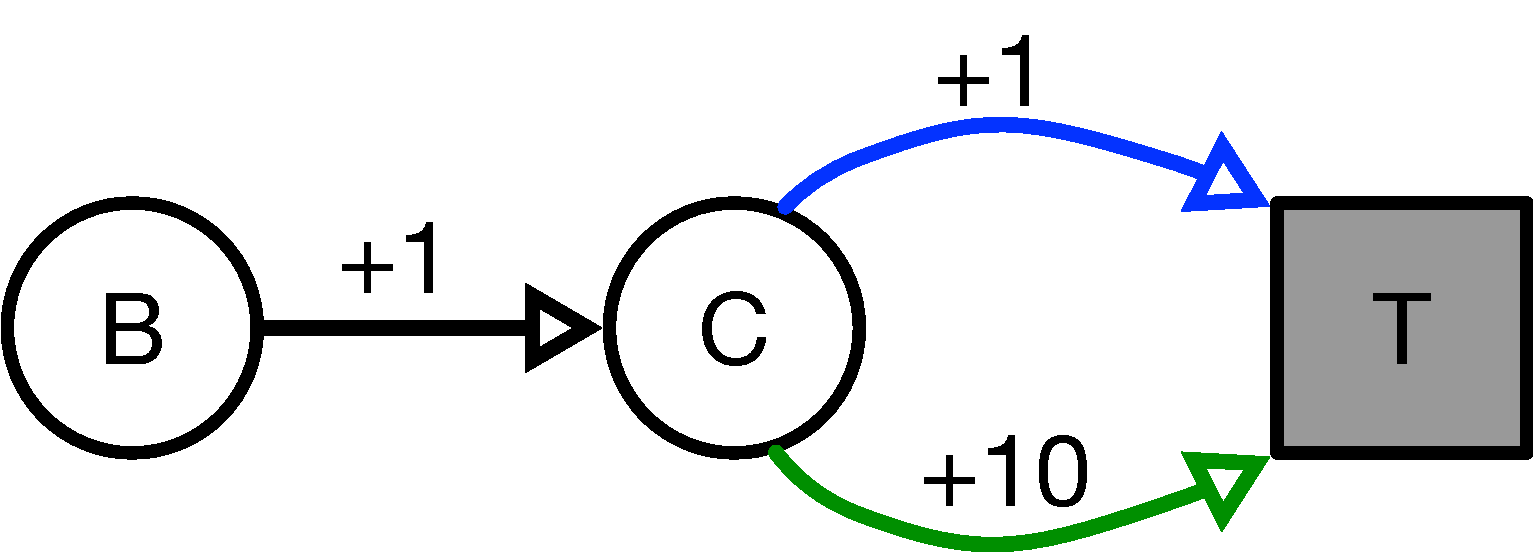
\includegraphics[width=0.5\linewidth]{figures/c2_2state.pdf}
\end{figure}

%%%%%%ANSWERS%%%%%%
% (a) vpi(C) = 1.9, vpi(B) = 2.9
% (b) Return is 2
% (c) Return is 11
% (d) Return is 1.47


